\chapter{Methodology}

This chapter proposes an interpretative framework for transformer language models based on the concept of movement through embedding space.

The core insight is to view transformer operation as a trajectory from token $t_i$ to token $t_{i+1}$ in the embedding space. This process begins at the embedding of token $t_i$ and proceeds through a series of transformations as $L$ decoder layers are applied sequentially. Each decoder layer contributes an additive shift to the residual stream, creating a piecewise linear path through the embedding space, as illustrated in Figure \ref{fig:transformer_residual_sream}.

\begin{figure}[h]
    \centering
    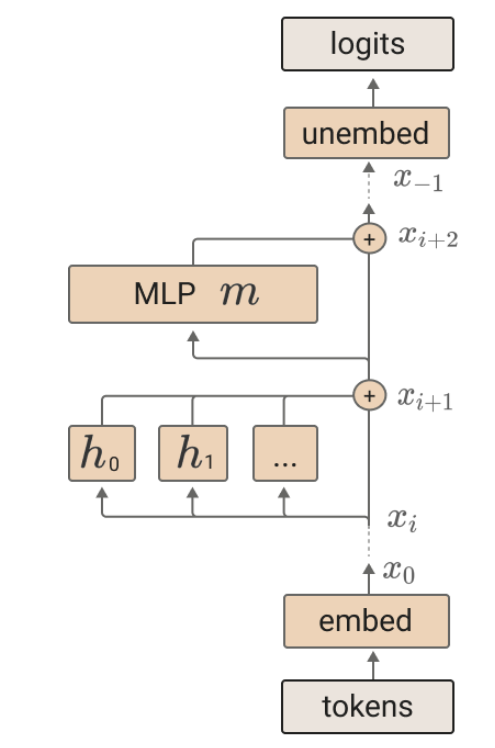
\includegraphics[height=0.5\textwidth]{images/residual_stream.png}
    \caption{Illustration of the decoder-only transformer operation from the residual flow perspective (adapted from \cite{math_framework_transformer}). In this illustration, intermediate hidden states are denoted as $x_0, x_1, \dots, x_{-1}$}
    \label{fig:transformer_residual_sream}
\end{figure}

After the final decoder layer produces the hidden state $\mathbf{h}_i^L$, the language modeling head generates a distribution over possible next tokens. The selection of token $t_{i+1}$ (via sampling or greedy selection) creates a "discontinuity" in the trajectory, as computation then continues from the embedding of this new token rather than from the final hidden state. Figure \ref{fig:my_transformer_schema} provides a simplified visualization of this token-to-token movement pattern.

\begin{figure}[h]
    \centering
    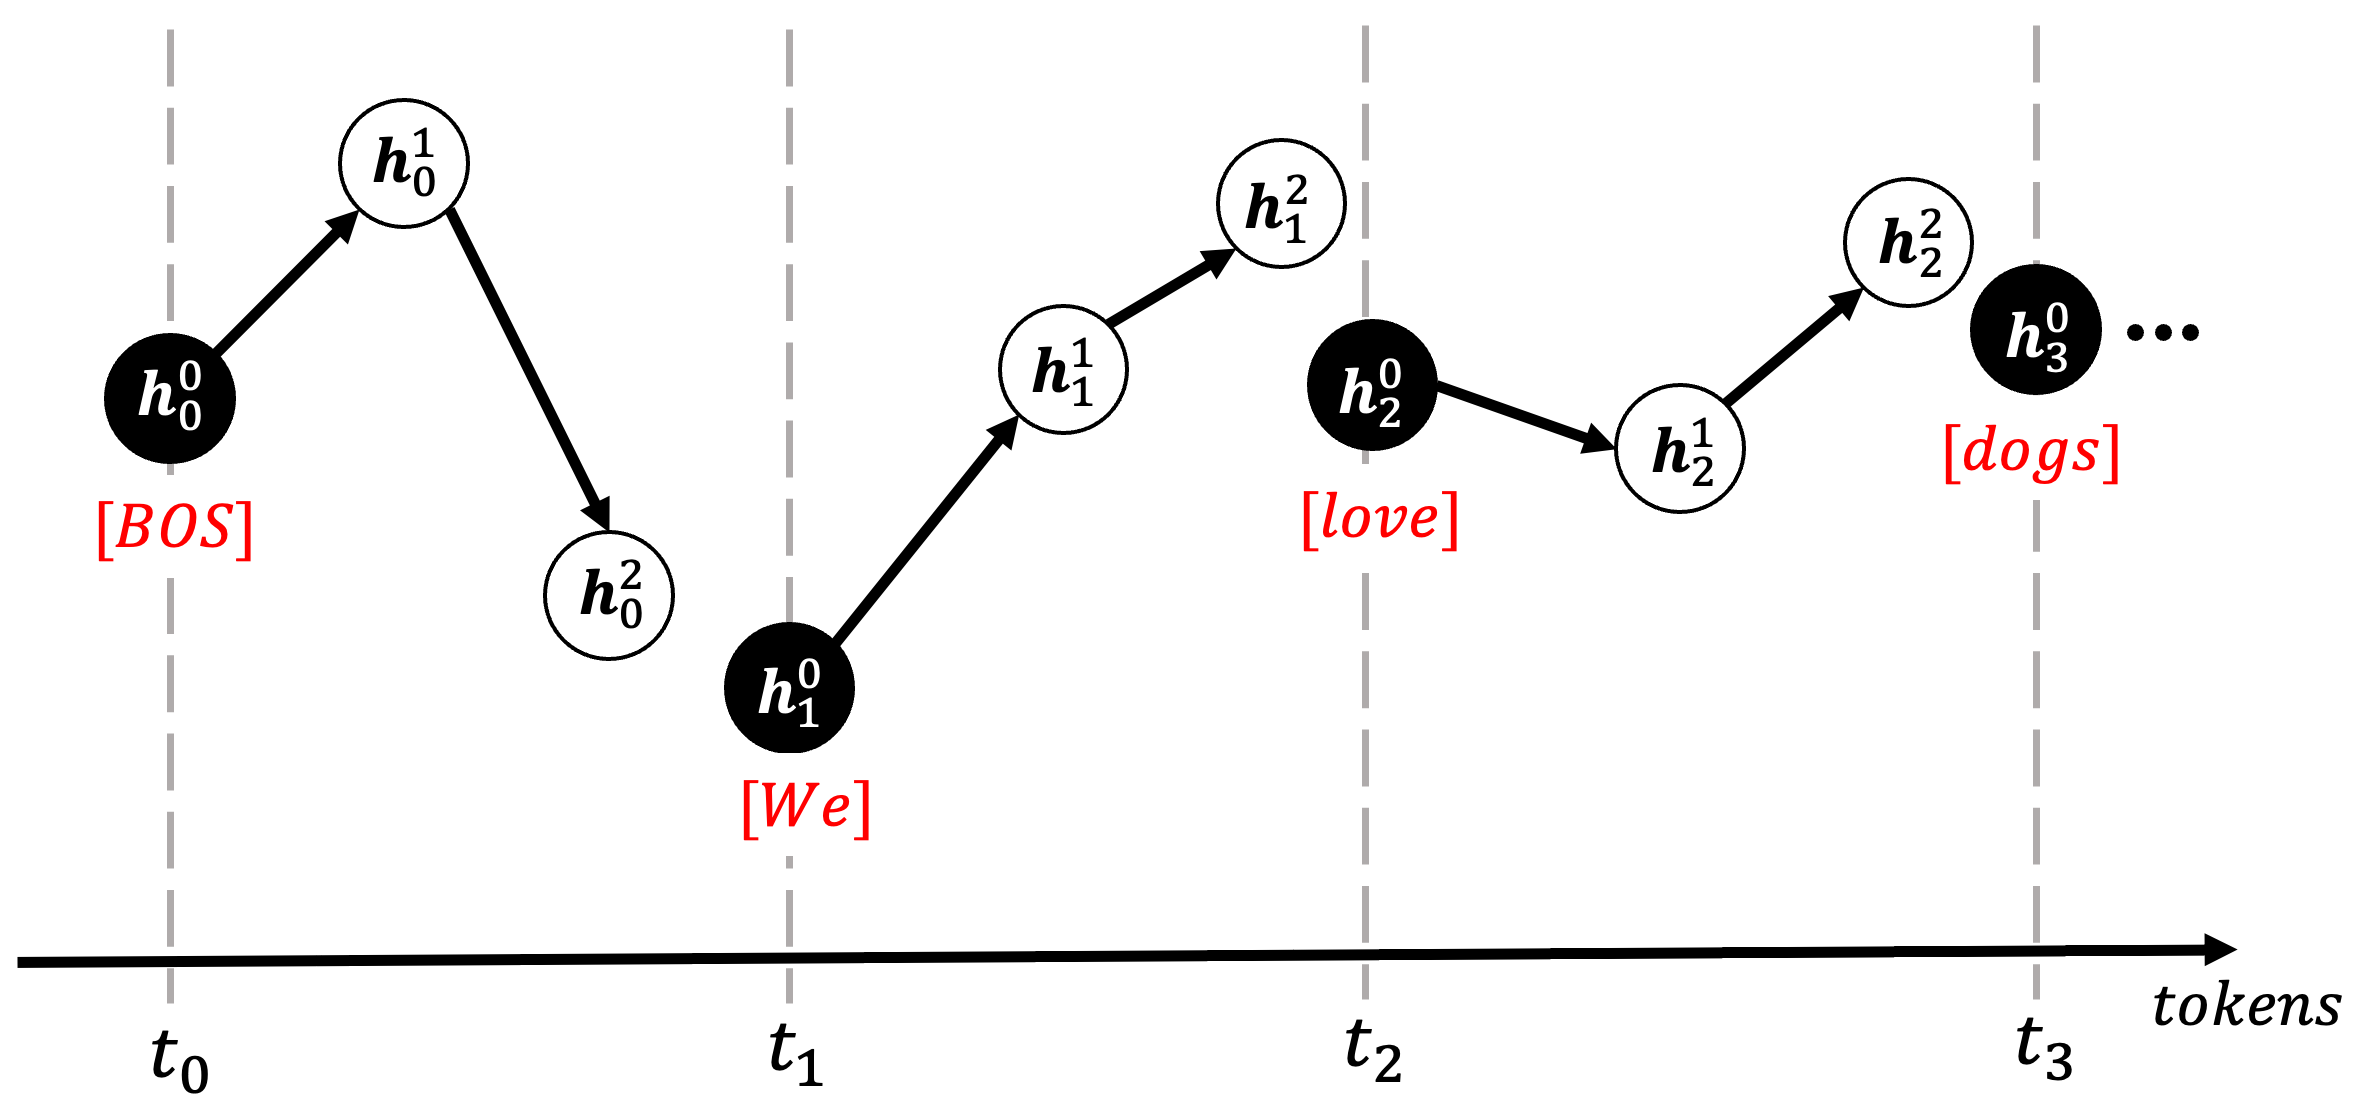
\includegraphics[width=0.75\textwidth]{images/my_transformer_schema_new.png}
    \caption{Simplified transformer operation diagram illustrating movement in embedding space. Filled circles represent token embeddings $t_{0}, t_{1}, \dots$, while empty circles represent intermediate hidden states $\mathbf{h}_0^0, \mathbf{h}_0^1, \mathbf{h}_1^0, \mathbf{h}_1^1, \dots$. The axis indicates the token sequence direction.}
    \label{fig:my_transformer_schema}
\end{figure}

To verify the applicability of the proposed interpretation to real transformers, the following analytical tools are suggested.

\section{Proximity Analysis Between Final Hidden States and Token Embeddings}\label{final_hidden_method}

A crucial aspect of the paradigm of movement in token embedding space is that the final hidden state should be close to the embedding of the next predicted token.

This behavior of the transformer can be visualized using the diagram in Figure \ref{fig:knn_schema}, which complements Figure \ref{fig:my_transformer_schema}.

\begin{figure}[h]
    \centering
    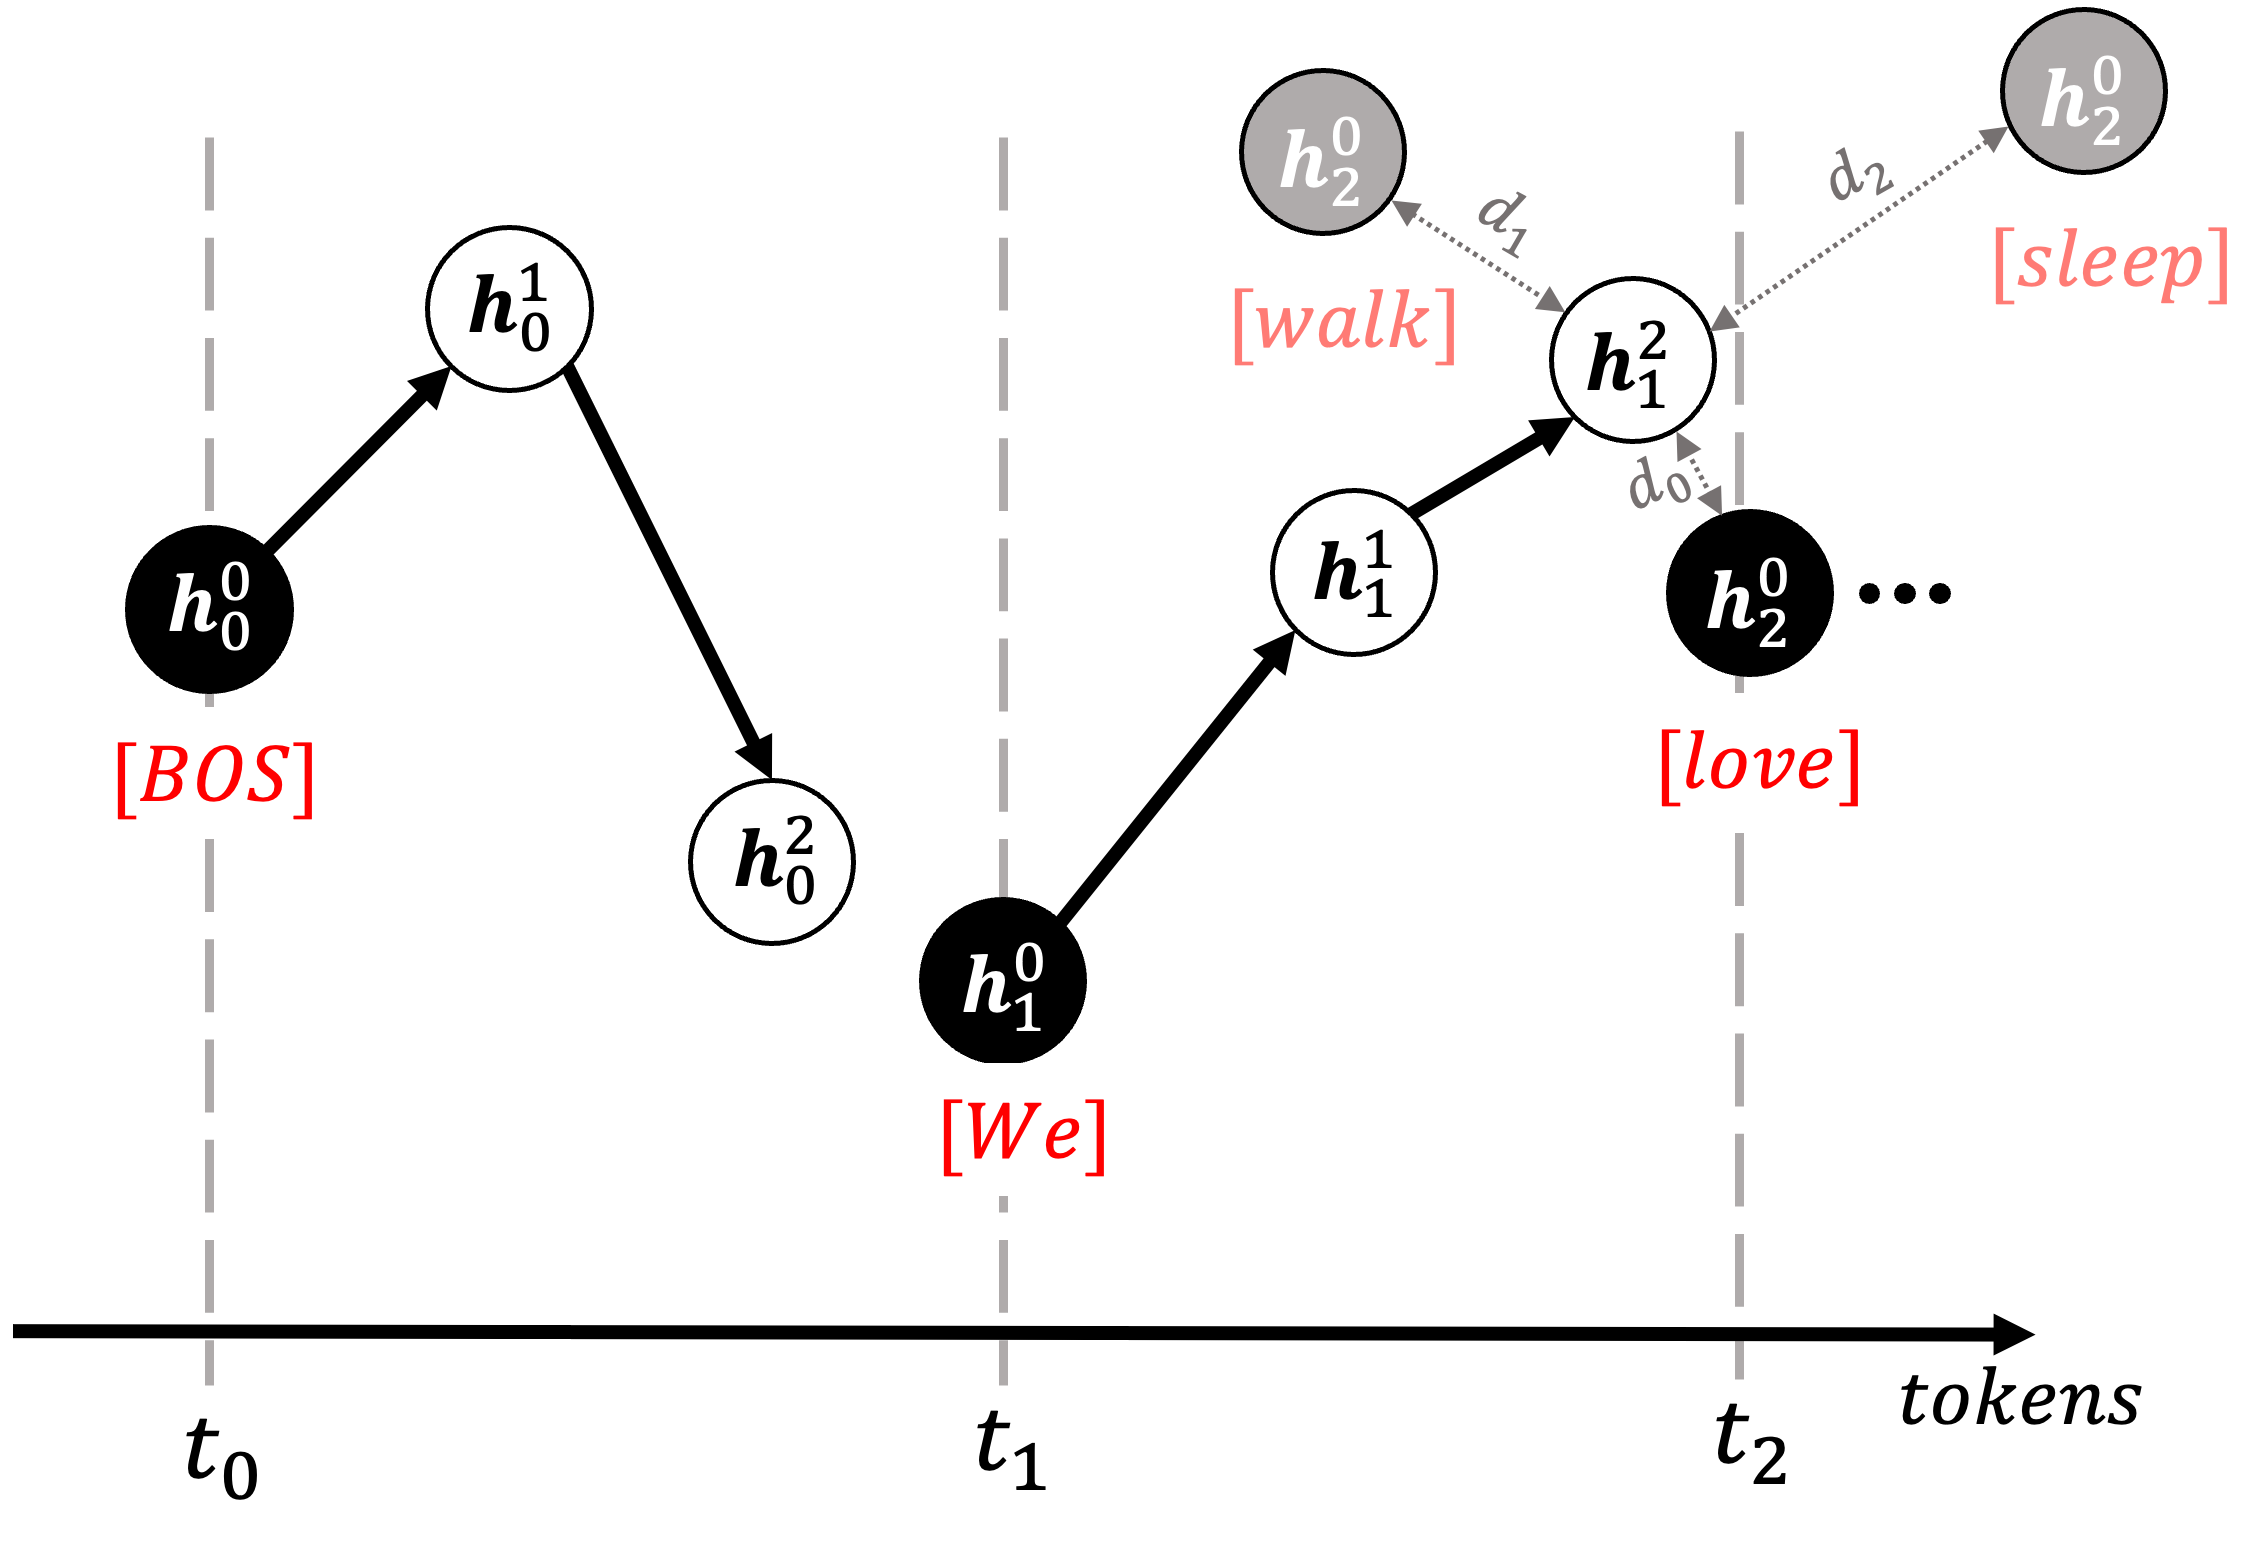
\includegraphics[width=0.6\textwidth]{images/knn_head_new.png}
    \caption{Illustration demonstrating the importance of proximity between the final hidden state $\mathbf{h}_i^L$ and the next token embedding $t_{i+1}$ in the proposed transformer interpretation paradigm. Distances is $d_j = \rho(h_1^2, t_j)$ and $d_0 < d_1 < d_2$.}
    \label{fig:knn_schema}
\end{figure}

To systematically evaluate this hypothesis, two complementary approaches are proposed: analyzing pre-trained transformers and training new models with specific constraints.

\subsection{Measuring Similarity Between Hidden States and Token Embeddings in Pre-trained Models}

To verify whether pre-trained transformers conform to this requirement, it is proposed to measure how well the distances between final hidden states and token embeddings correlate with the token probabilities predicted by the language modeling head for these same hidden states.

For this purpose, it is necessary to introduce a similarity metric between the final hidden state and all token embeddings in the model's vocabulary.

The first metric is Euclidean similarity. To measure this, the Euclidean distances are first calculated and then inverted by negation or taking the reciprocal:

\begin{equation}
d_{\text{Euclid}}(\mathbf{h}_i^L, \mathbf{e}_j) = \|\mathbf{h}_i^L - \mathbf{e}_j\|_2
\end{equation}

\begin{equation}
\text{sim}_{\text{NegEuclid}}(\mathbf{h}_i^L, \mathbf{e}_j) = -d_{\text{Euclid}}(\mathbf{h}_i^L, \mathbf{e}_j)
\end{equation}

\begin{equation}
\text{sim}_{\text{InvEuclid}}(\mathbf{h}_i^L, \mathbf{e}_j) = \frac{1}{d_{\text{Euclid}}(\mathbf{h}_i^L, \mathbf{e}_j)}
\end{equation}

Additionally, two other similarity metrics are considered: cosine similarity and dot similarity:

\begin{equation}
\text{sim}_{\text{cosine}}(\mathbf{h}_i^L, \mathbf{e}_j) = \frac{\mathbf{h}_i^L \cdot \mathbf{e}_j}{\|\mathbf{h}_i^L\|_2 \|\mathbf{e}_j\|_2}
\end{equation}

\begin{equation}
\text{sim}_{\text{dot}}(\mathbf{h}_i^L, \mathbf{e}_j) = \mathbf{h}_i^L \cdot \mathbf{e}_j = \sum_{k=1}^{d} h_{i,k}^L e_{j,k}
\end{equation}

To evaluate the alignment between model predictions and embedding space proximity, the correlation between language model logits and the similarity metrics is measured. This comparison employs the Normalized Discounted Cumulative Gain (NDCG), a standard metric for ranking quality assessment:

\begin{equation}
\text{NDCG@k} = \frac{\text{DCG@k}}{\text{IDCG@k}}
\end{equation}

where DCG@k (Discounted Cumulative Gain) is defined as:

\begin{equation}
\text{DCG@k} = \sum_{i=1}^{k} \frac{2^{\text{rel}_i} - 1}{\log_2(i+1)}
\end{equation}

Here, $\text{rel}_i$ is the relevance score of the item at position $i$, and IDCG@k is the DCG@k value for the ideal ranking. In this context, the relevance scores are derived from the token probabilities predicted by the language modeling head, and the comparison evaluates how well the similarity metrics align with these probabilities.

\subsection{Constructing Similarity-Based Language Modeling Heads for New Models}\label{scratch_final_hidden_info}

It is possible to attempt training a transformer with the desired properties from scratch. To do this, it is necessary to explicitly construct logits based on the proximity of the final hidden state to token embeddings.

For the case of dot similarity, such a construction method is well-known and is called weight tying. By tying the weight matrix in the language modeling head to the embedding matrix of the model, dot similarity is explicitly calculated as logits at the output of the language modeling head layer:

\begin{equation}
\text{LmHead}_{tied}(\mathbf{h}_i^L) = \mathbf{E} \mathbf{h}_i^L + \mathbf{b} = [\text{sim}_{\text{dot}}(\mathbf{h}_i^L, \mathbf{e}_1) + b_1, \ldots, \text{sim}_{\text{dot}}(\mathbf{h}_i^L, \mathbf{e}_{|\mathcal{V}|}) + b_{|\mathcal{V}|}]
\end{equation}

where $\mathbf{E} \in \mathbb{R}^{|\mathcal{V}| \times d}$ is the embedding matrix containing token embeddings $\mathbf{e}_j$, $\mathbf{h}_i^L \in \mathbb{R}^d$ is the final hidden state, and $\mathbf{b} \in \mathbb{R}^{|\mathcal{V}|}$ is the bias vector.

The Euclidean metric can also be approached in a similar manner. This involves simply outputting distances with a negative sign as logits at the layer output. Negation is chosen for simpler computation during training (inverting the distance is a more expensive operation). Such a layer is termed KnnHead:

\begin{equation}
\text{KnnHead}(\mathbf{h}_i)_j = \text{sim}_{\text{NegEuclid}}(\mathbf{h}_i^L, \mathbf{e}_j) + b_j = -\|\mathbf{h}_i^L - \mathbf{e}_j\|_2^2 + b_j
\end{equation}

Note that the squared Euclidean distance is used for computational efficiency, as it preserves the same ordering of distances while avoiding the square root operation.

Cosine similarity is not utilized as a head function when training transformers from scratch in this framework.

\section{Analyzing Intermediate Hidden States in Embedding Space}\label{reg_info}

Beyond the proximity of the final hidden state to the next token, the position of all intermediate hidden states is also crucial in this interpretative framework. It is logical to expect that intermediate hidden states should reside somewhere in the vicinity of the vocabulary token embeddings, since the transformer's movement in this paradigm occurs specifically from token to token.

For studying the position of intermediate hidden states in pre-trained transformers, the simplest approach is to examine their norms and visualize how these norms change depending on the layer number or the token position in the sentence. Heatmap visualizations of these norm patterns will be presented in the numerical experiments section.


When training a transformer from scratch, it is possible to explicitly penalize the model when certain intermediate hidden states deviate too far from the cloud of token embedding points. This can be implemented through a regularizer that linearly penalizes those intermediate hidden states whose norm exceeds the mean norm of token embeddings plus one and half standard deviations:

\begin{align}
    \mathcal{R}(\mathbf{h}_i^l) &= \lambda \cdot \max(0, \|\mathbf{h}_i^l\|_2 - (\mu_{\mathbf{E}} + \frac{3}{2} \sigma_{\mathbf{E}})) \\
    \mu_{\mathbf{E}} &= \frac{1}{|\mathcal{V}|}\sum_{j=1}^{|\mathcal{V}|}\|\mathbf{e}_j\|_2 \\ 
    \sigma_{\mathbf{E}} &= \sqrt{\frac{1}{|\mathcal{V}|}\sum_{j=1}^{|\mathcal{V}|}(\|\mathbf{e}_j\|_2 - \mu_{\mathbf{E}})^2}
\end{align}

where $\mathcal{R}(\mathbf{h}_i^l)$ is the regularization penalty for hidden state $\mathbf{h}_i^l$, $\lambda$ is the regularization coefficient, and $\|\mathbf{h}_i^l\|_2$ is the L2 norm of the hidden state. The total regularization term would be the average of penalties across all hidden states and tokens:

\begin{equation}
\mathcal{R}_{\text{total}} = \frac{1}{n \cdot L} \cdot \sum_{i=1}^{n} \sum_{l=1}^{L} \mathcal{R}(\mathbf{h}_i^l)
\end{equation}

This regularization encourages intermediate hidden states to remain within a reasonable distance from the token embedding cloud, reinforcing the concept of movement through embedding space.
